% ============================================================
%  MANUAL BOOK -- PETUNJUK PENGGUNAAN APLIKASI DALSILENS
%  Dokumen terpisah dari Penulisan Ilmiah (main.tex), dapat
%  di-compile sendiri: pdflatex/latexmk manual.tex
%  Format mengikuti contoh "Manual Book RCC PI" dari dosen:
%  judul section polos (tanpa nomor bab), cover berbanner,
%  Daftar Isi manual sederhana, langkah pakai bernomor+huruf.
% ============================================================
\documentclass[12pt, a4paper]{article}

\usepackage[utf8]{inputenc}
\usepackage[T1]{fontenc}
\usepackage{mathptmx}          % Times New Roman
\usepackage[bahasa]{babel}
\usepackage{geometry}
\usepackage{setspace}
\usepackage{graphicx}
\usepackage{float}
\usepackage{enumitem}
\usepackage{xcolor}
\usepackage{fancyhdr}
\usepackage{tikz}
\usepackage[hidelinks]{hyperref}
\usepackage{indentfirst}

% ----- Margin: samakan dengan Penulisan Ilmiah (4/3/4/3 cm A4) -----
\geometry{a4paper, top=4cm, bottom=3cm, left=4cm, right=3cm}
\graphicspath{{../gambar/}{image/}}

\setstretch{1.5}
\tolerance=1000
\emergencystretch=3em

% ----- Judul section: bold, tengah, tanpa nomor (mengikuti contoh) -----
\newcommand{\seksi}[1]{%
  \vspace{1em}
  \begin{center}{\bfseries\fontsize{14}{16}\selectfont #1}\end{center}
  \vspace{0.8em}
}
% ----- Sub-judul: bold, rata kiri, tanpa nomor -----
\newcommand{\subseksi}[1]{%
  \vspace{0.5em}
  {\bfseries\fontsize{12}{14}\selectfont #1}
  \vspace{0.3em}\par
}
% ----- Baris Daftar Isi: judul, garis titik-titik, nomor halaman -----
\newcommand{\tocline}[2]{%
  \noindent #1\dotfill #2\par
  \vspace{0.6em}
}

% ----- Header & footer: nomor halaman tengah bawah -----
\pagestyle{fancy}
\fancyhf{}
\fancyfoot[C]{\thepage}
\renewcommand{\headrulewidth}{0pt}
\fancypagestyle{plain}{
  \fancyhf{}
  \fancyfoot[C]{\thepage}
  \renewcommand{\headrulewidth}{0pt}
}

% ============================================================
%  DATA
% ============================================================
\newcommand{\NamaMahasiswa}{Anaf Naufalian}
\newcommand{\NPM}{50423155}
\newcommand{\JudulAplikasi}{DALSILENS: ALAT BANTU MOBILE REAL-TIME UNTUK PENDERITA DIKROMASI MENGGUNAKAN DALTONISASI LMS DAN IDENTIFIKASI WARNA BERBASIS HSV}
\newcommand{\Tahun}{2026}

\begin{document}

% ============================================================
%  COVER (dengan banner biru, mengikuti contoh)
% ============================================================
\thispagestyle{empty}
\begin{tikzpicture}[remember picture, overlay]
  \shade[left color=blue!12, right color=blue!55]
    (current page.north west) rectangle
    ([yshift=-3.2cm]current page.north east);
  \node[anchor=west, text=black, font=\bfseries\fontsize{30}{34}\selectfont]
    at ([xshift=1.3cm, yshift=-1.6cm]current page.north west)
    {PETUNJUK PENGGUNAAN};
\end{tikzpicture}

\vspace{2.8cm}

\begin{center}
  {\bfseries\fontsize{20}{24}\selectfont APLIKASI \JudulAplikasi}

  \vspace{1cm}
  
\includegraphics[width=6cm]{logo-gundar}
  \vspace{2cm}

  {\fontsize{16}{19}\selectfont Dibuat oleh:}\\[0.2cm]
  {\bfseries\fontsize{16}{19}\selectfont \NamaMahasiswa\ }

  \vfill
  {\bfseries\fontsize{20}{24}\selectfont UNIVERSITAS GUNADARMA}\\[0.3cm]
  {\bfseries\fontsize{20}{24}\selectfont \Tahun}
\end{center}
\newpage

% ============================================================
%  DAFTAR ISI (manual sederhana, mengikuti contoh -- bukan
%  \tableofcontents otomatis)
% ============================================================
\setcounter{page}{2}
\seksi{Daftar Isi}
\vspace{1em}
\tocline{Cover}{i}
\tocline{Daftar Isi}{ii}
\tocline{Gambaran Umum Aplikasi}{iii}
\tocline{Kebutuhan Hardware dan Software}{iv}
\tocline{Arsitektur Aplikasi (Ringkasan Teknis)}{v}
\tocline{Petunjuk Penggunaan}{vi}
\newpage

% ============================================================
\seksi{Gambaran Umum}
% ============================================================

Dalsilens merupakan aplikasi \textit{mobile} berbasis Android yang dirancang
untuk membantu penderita dikromasi (\textit{Color Vision Deficiency} tipe
Protanopia, Deuteranopia, dan Tritanopia) dalam membedakan warna secara
\textit{real-time} melalui kamera \textit{smartphone}. Aplikasi ini
menggunakan algoritma Daltonisasi LMS yang mengonversi citra dari kamera ke
ruang warna LMS untuk menggeser informasi warna yang tidak dapat dibedakan
penderita, sekaligus fitur identifikasi nama warna berbasis ruang warna HSV
yang mengklasifikasikan warna objek secara tekstual. Kedua fitur berjalan
langsung pada perangkat (\textit{on-device}) tanpa memerlukan koneksi
internet, sehingga latensinya rendah dan dapat digunakan kapan saja. Aplikasi
ini hanya berfungsi sebagai alat bantu visual, bukan pengganti diagnosis
medis dari tenaga profesional.
\newpage

% ============================================================
\seksi{Kebutuhan Perangkat}
% ============================================================

\subseksi{Perangkat Keras}
Spesifikasi minimal dari komponen perangkat keras yang dibutuhkan untuk
menjalankan aplikasi Dalsilens adalah sebagai berikut:
\begin{enumerate}
  \item \textit{Smartphone} berbasis Android dengan kamera belakang yang
        berfungsi dengan baik.
  \item RAM minimal 3 GB agar pemrosesan citra secara \textit{real-time}
        berjalan lancar.
\end{enumerate}

\subseksi{Perangkat Lunak}
Spesifikasi minimal dari komponen perangkat lunak yang dibutuhkan untuk
menjalankan aplikasi adalah sebagai berikut:
\begin{enumerate}
  \item Sistem operasi Android versi 8.0 (Oreo, API level 26) atau lebih
        baru.
  \item Izin (\textit{permission}) akses kamera yang disetujui pengguna
        pada saat aplikasi pertama kali dijalankan.
\end{enumerate}
\newpage

% ============================================================
\seksi{Arsitektur Aplikasi (Ringkasan Teknis)}
% ============================================================

Bagian ini memberikan ringkasan teknis bagi pengembang lain yang ingin
memahami atau melanjutkan pengembangan aplikasi Dalsilens. Gambar~1
menunjukkan hubungan antar komponen utama sistem yaitu modul akuisisi citra
(CameraX), modul pemrosesan warna (\texttt{ColorProcessor}), dan modul
identifikasi nama warna (\texttt{ColorNames}).

\begin{center}
  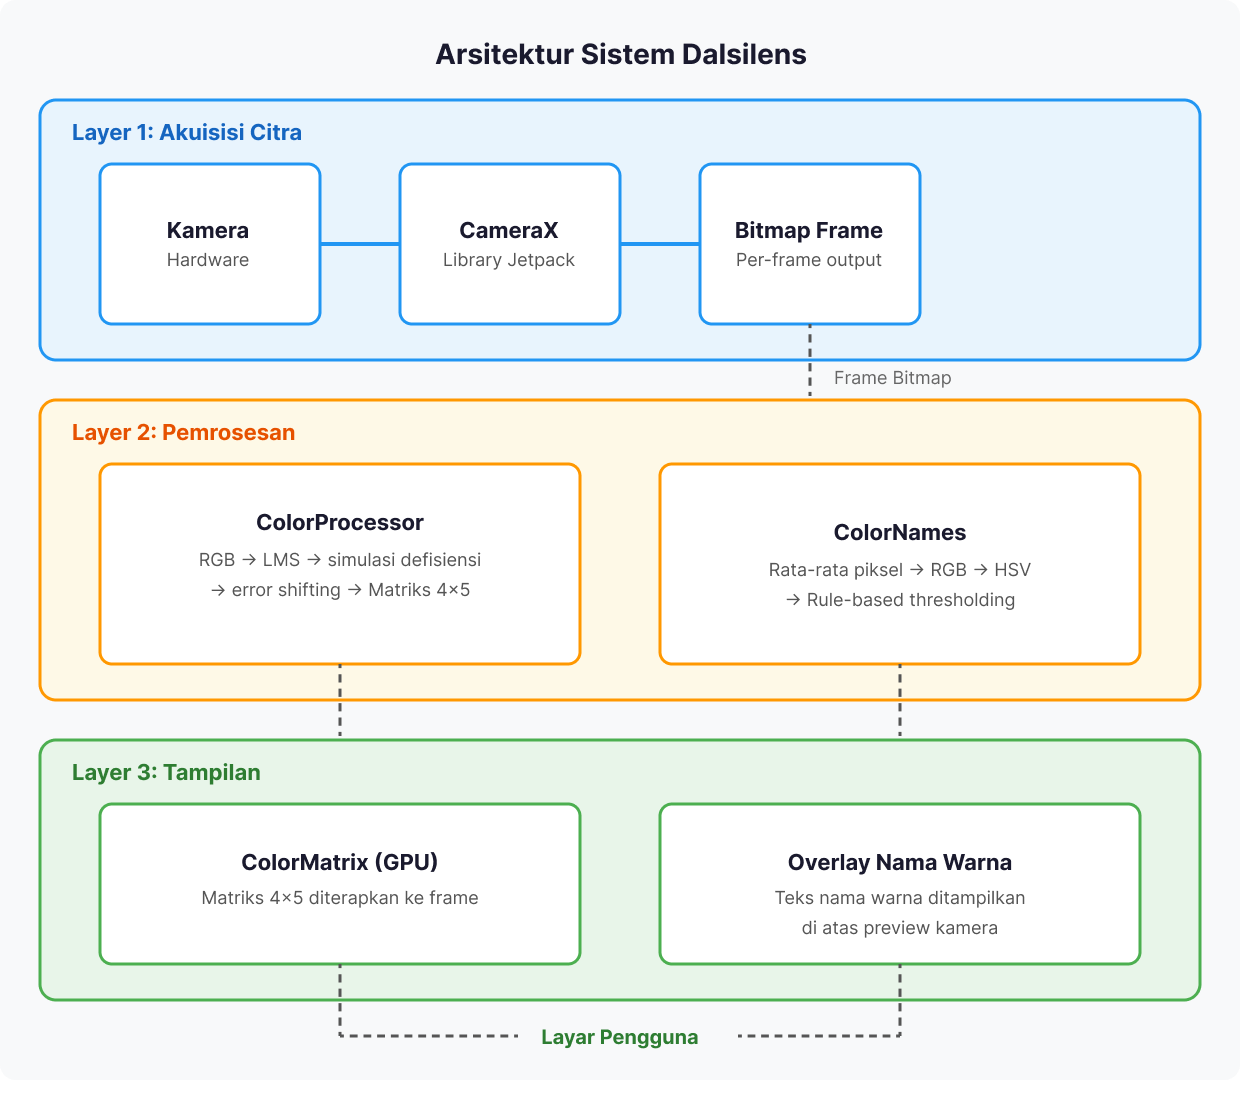
\includegraphics[width=0.9\textwidth]{arsitektur-umum}\\[0.3em]
  \textit{Gambar 1. Arsitektur umum aplikasi Dalsilens}
\end{center}

Tiga kelas Kotlin berikut menjadi inti pemrosesan aplikasi.
\begin{itemize}
  \item \texttt{ColorProcessor}: mengonversi RGB ke ruang warna LMS,
        mensimulasikan defisiensi warna, dan membangun matriks transformasi
        $4\times5$ untuk simulasi maupun daltonisasi yang diterapkan langsung
        pada \texttt{ColorFilter} Android.
  \item \texttt{ColorNames}: mengambil rata-rata warna piksel di sekitar
        titik tengah layar, lalu mengklasifikasikan nama warnanya
        berdasarkan nilai \textit{Hue}, \textit{Saturation}, dan
        \textit{Value}.
  \item \texttt{CameraScreen}: menginisialisasi CameraX (\textit{preview}
        dan \textit{image analysis}) serta menjalankan analisis pada setiap
        \textit{frame} kamera secara \textit{real-time}.
\end{itemize}
\newpage

% ============================================================
\seksi{Petunjuk Penggunaan}
% ============================================================

Berikut adalah petunjuk untuk menggunakan aplikasi Dalsilens:
\begin{enumerate}
\item Pasang berkas APK aplikasi Dalsilens pada perangkat Android, lalu
      izinkan permintaan akses kamera (\textit{Camera Permission}) saat
      aplikasi pertama kali dijalankan.

\begin{enumerate}[label=\alph*)]

\item Tampilan halaman \textit{Dashboard}. Untuk masuk ke halaman kamera dan
      melakukan simulasi, ketuk tombol \textbf{``Go To Camera''}.
\begin{figure}[H]
  \centering
  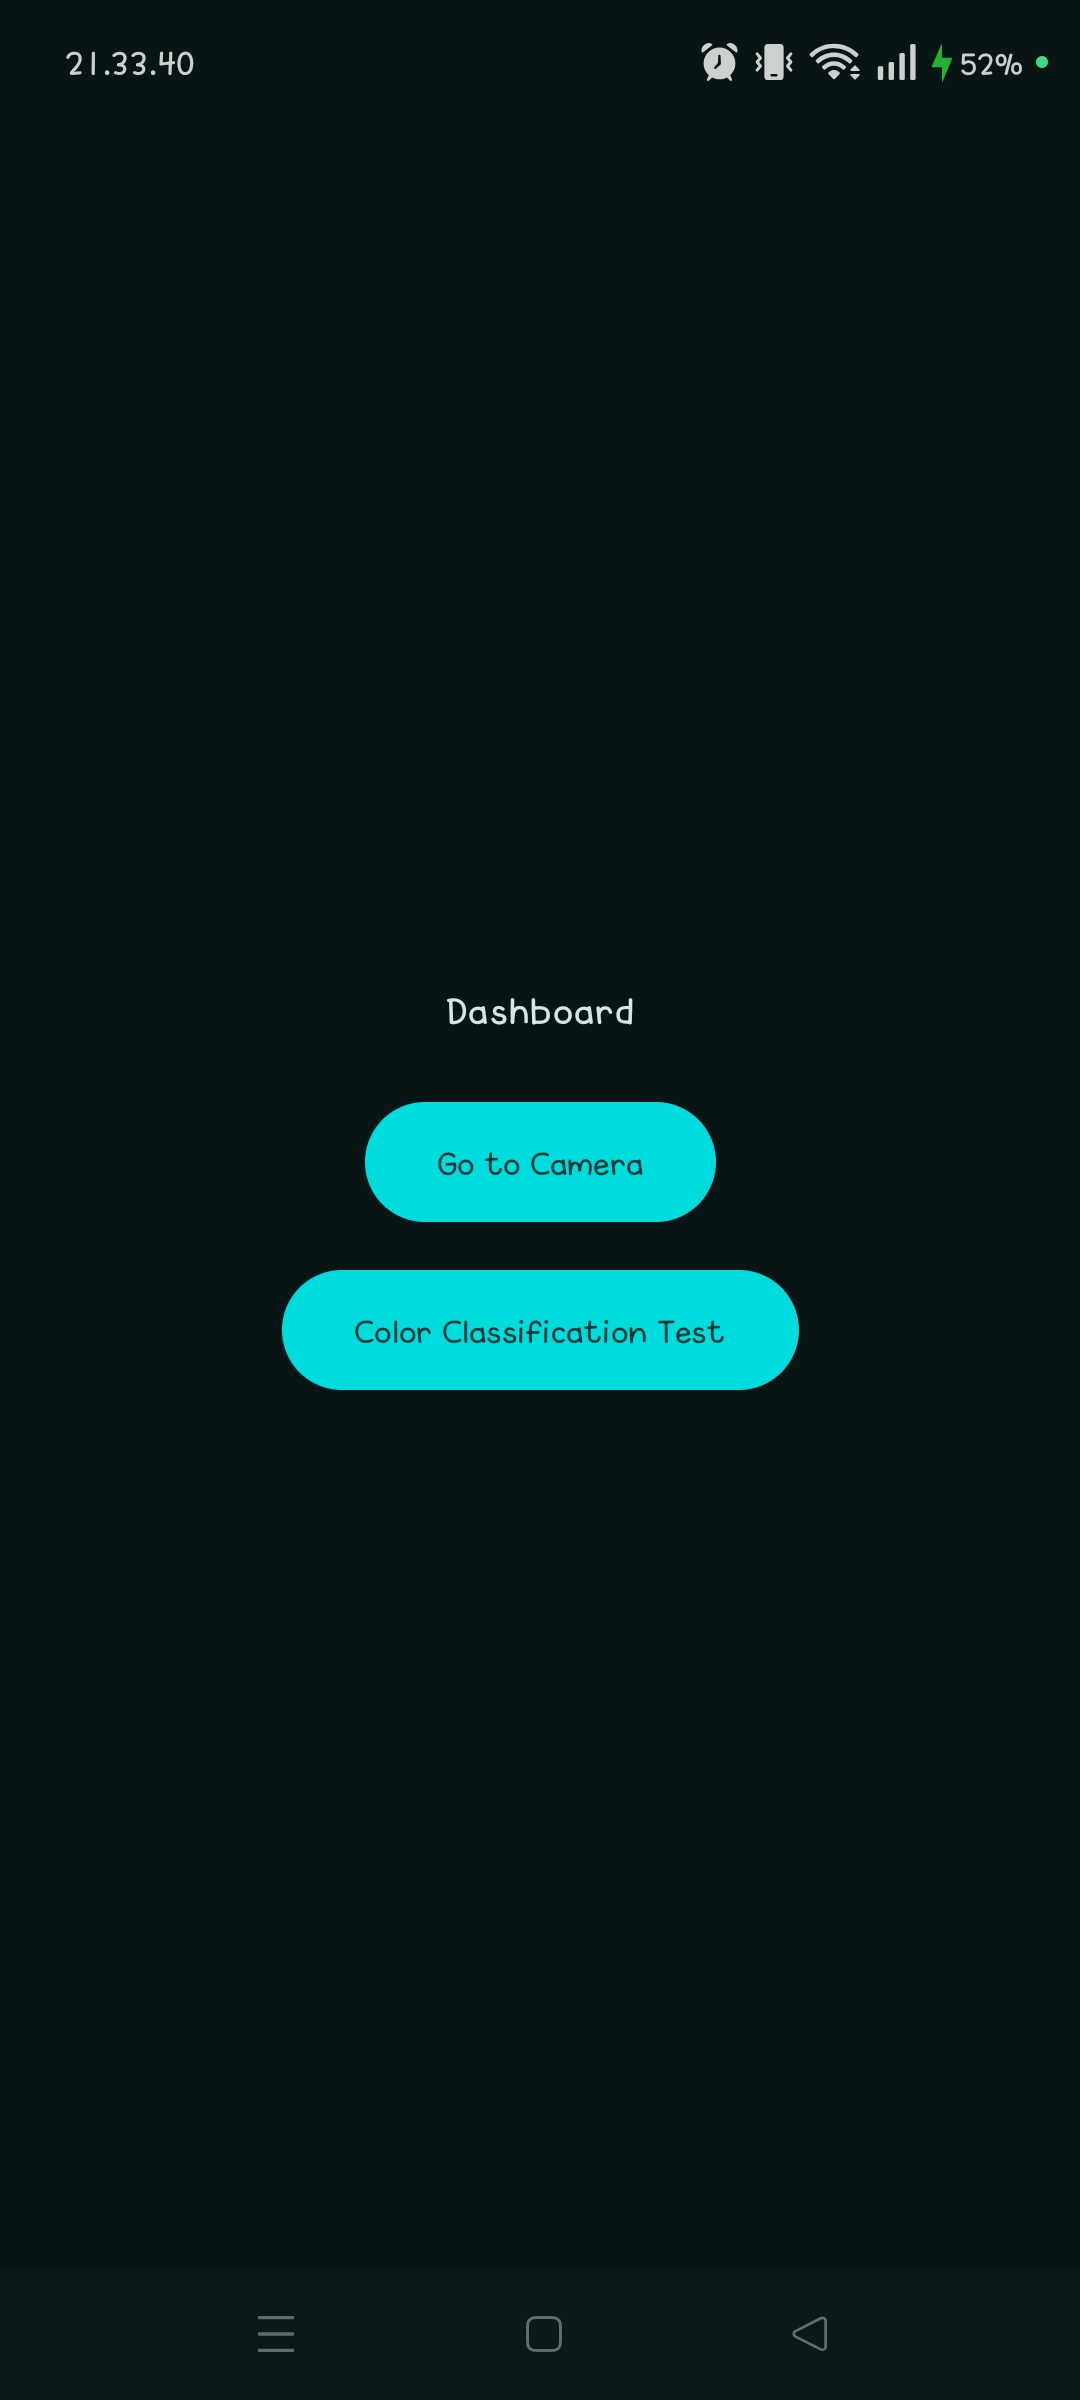
\includegraphics[width=0.35\textwidth]{ss_dashboard}
\end{figure}
\vspace{-0.5em}

Pada halaman kamera, ketuk ikon \textit{magic wand} di sisi kanan layar
untuk membuka panel \textbf{Filter Settings}, yang berisi pengaturan
berikut:
\begin{itemize}
  \item \textbf{Enable Daltonization}: tombol untuk mengaktifkan atau
        menonaktifkan filter daltonisasi pada \textit{preview} kamera.
  \item \textbf{Simulation Type}: memilih jenis simulasi dikromasi yang
        ingin ditampilkan yaitu \textit{Normal}, \textit{Protanopia},
        \textit{Deuteranopia}, atau \textit{Tritanopia}.
  \item \textbf{Severity}: \textit{slider} untuk mengatur intensitas
        simulasi/koreksi warna, bernilai 0 (tanpa efek) hingga 1 (efek
        penuh).
  \item \textbf{Sample Area Size}: mengatur radius area piksel yang
        diambil sampelnya di titik tengah layar untuk identifikasi warna.
\end{itemize}

\noindent
\begin{minipage}[t]{0.48\linewidth}
  \centering
  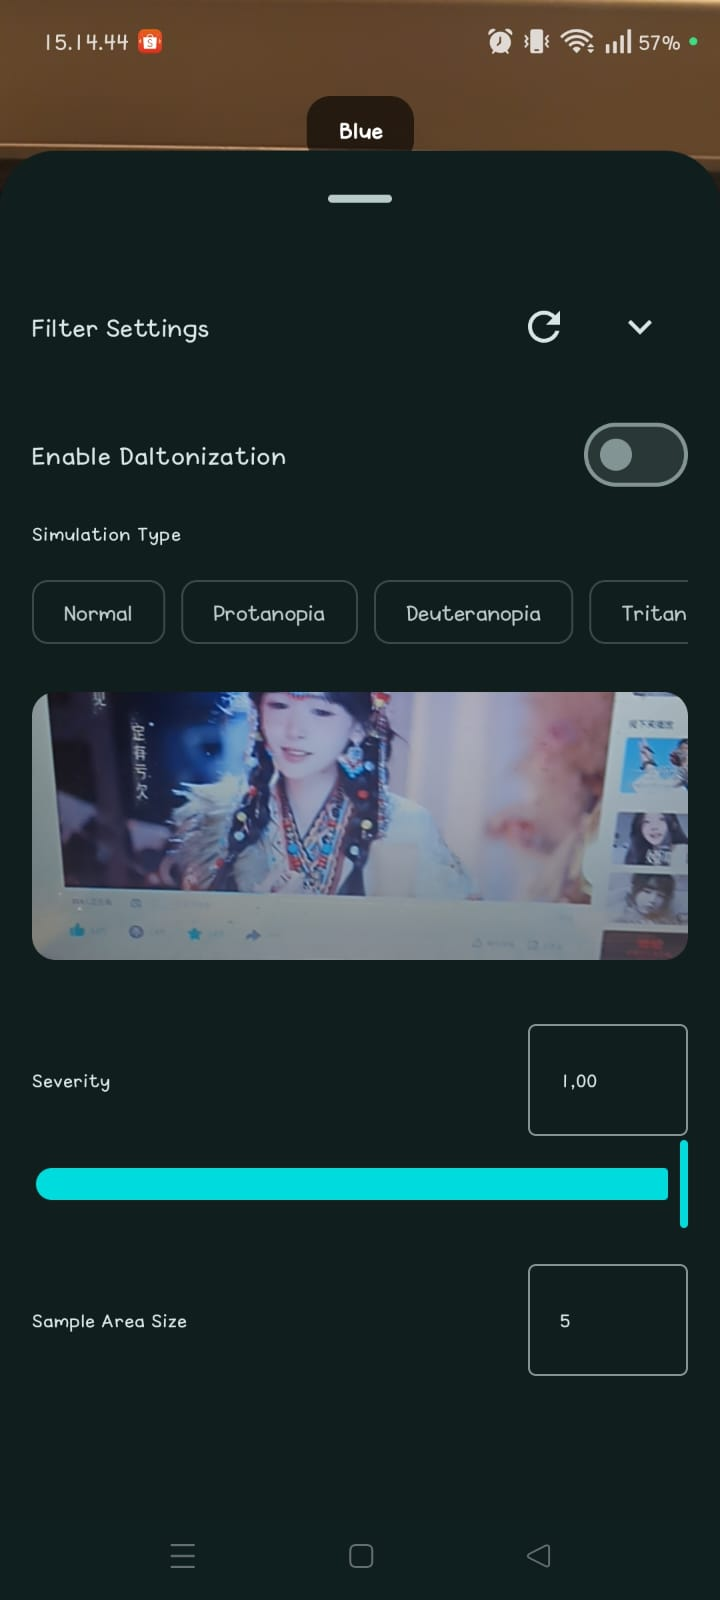
\includegraphics[width=\linewidth]{1}\\[0.2em]
  \textit{Panel Filter Settings}
\end{minipage}
\hfill
\begin{minipage}[t]{0.48\linewidth}
  \centering
  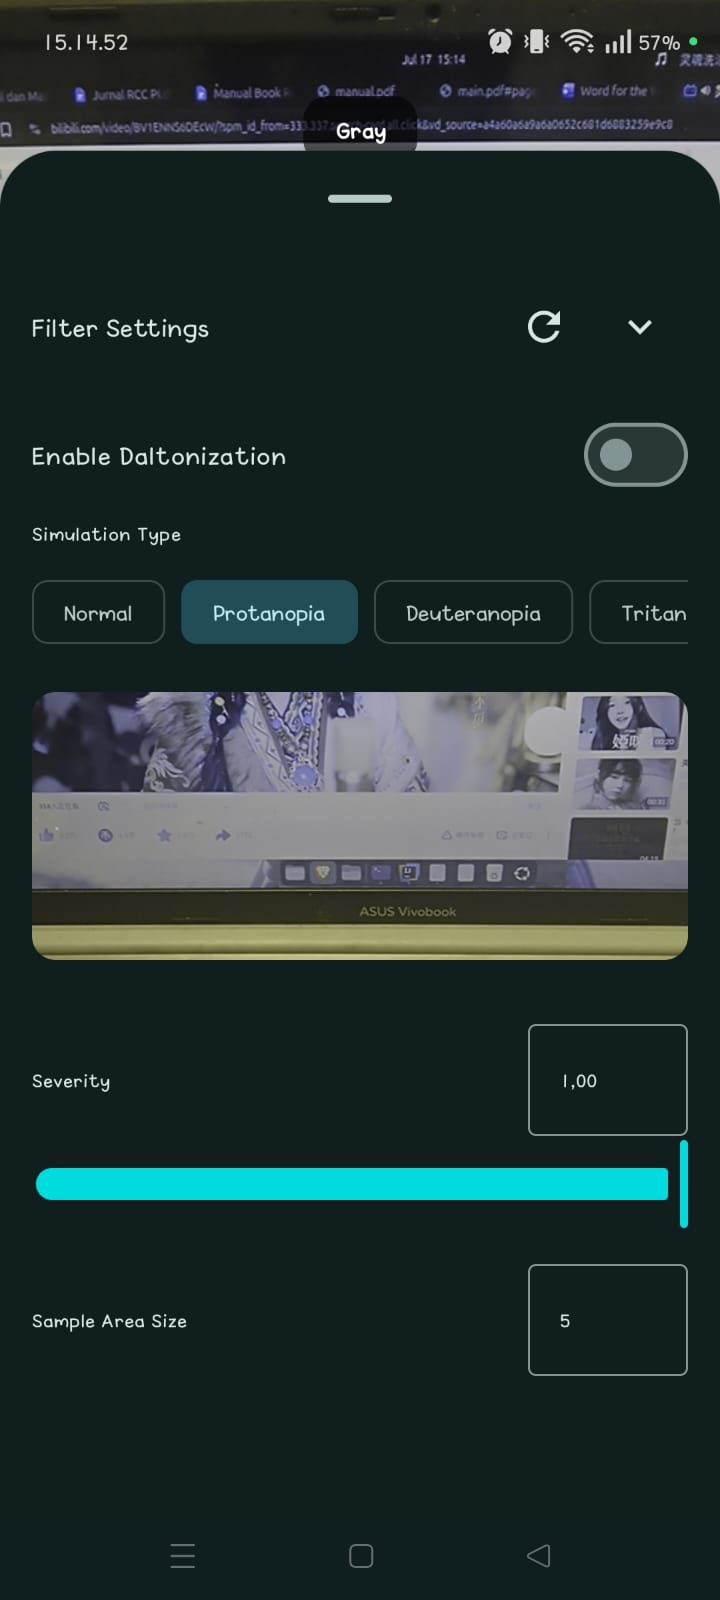
\includegraphics[width=\linewidth]{2}\\[0.2em]
  \textit{Simulation Type: Protanopia}
\end{minipage}
\vspace{1em}

\noindent
\begin{minipage}[t]{0.48\linewidth}
  \centering
  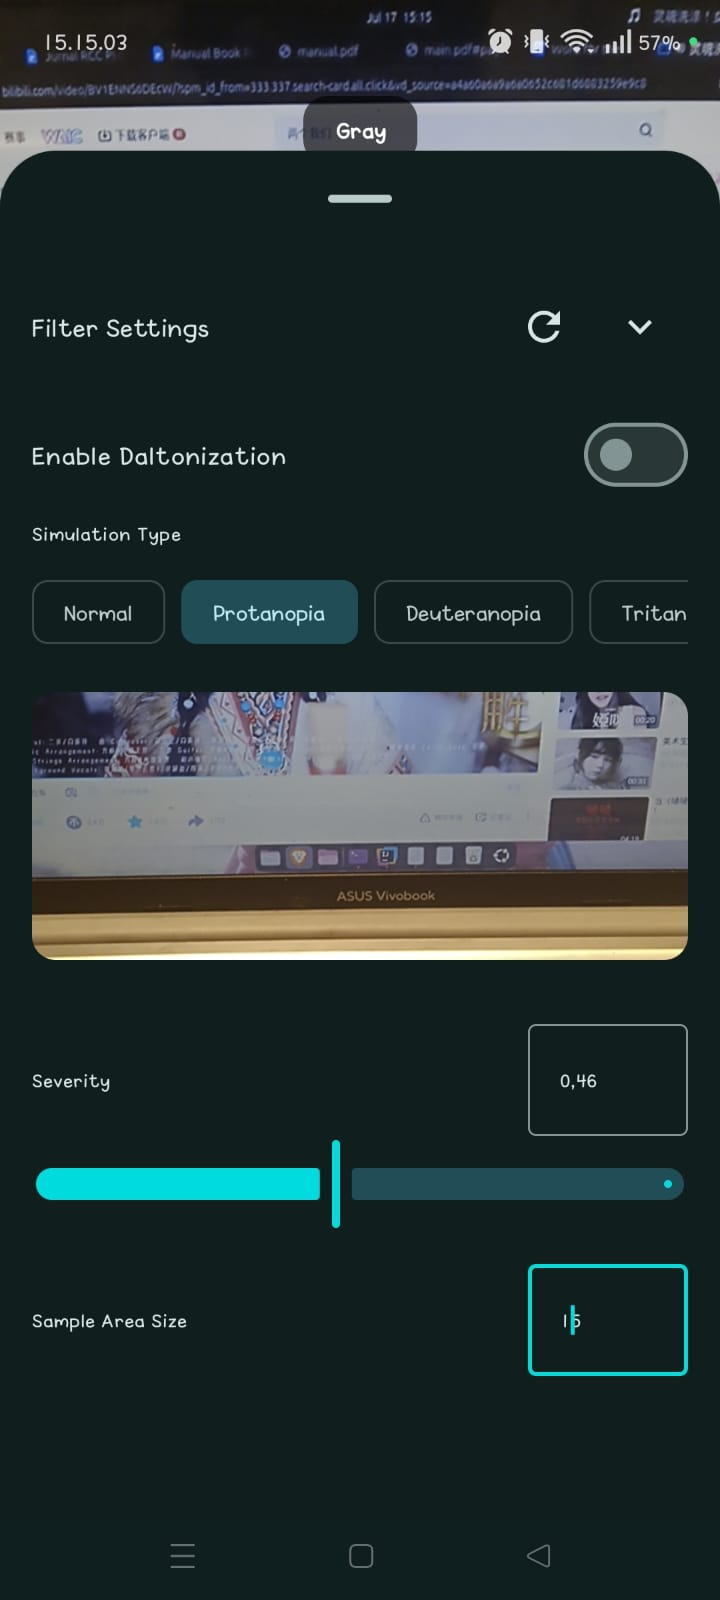
\includegraphics[width=\linewidth]{3}\\[0.2em]
  \textit{Mengatur Severity dan Sample Area Size}
\end{minipage}
\hfill
\begin{minipage}[t]{0.48\linewidth}
  \centering
  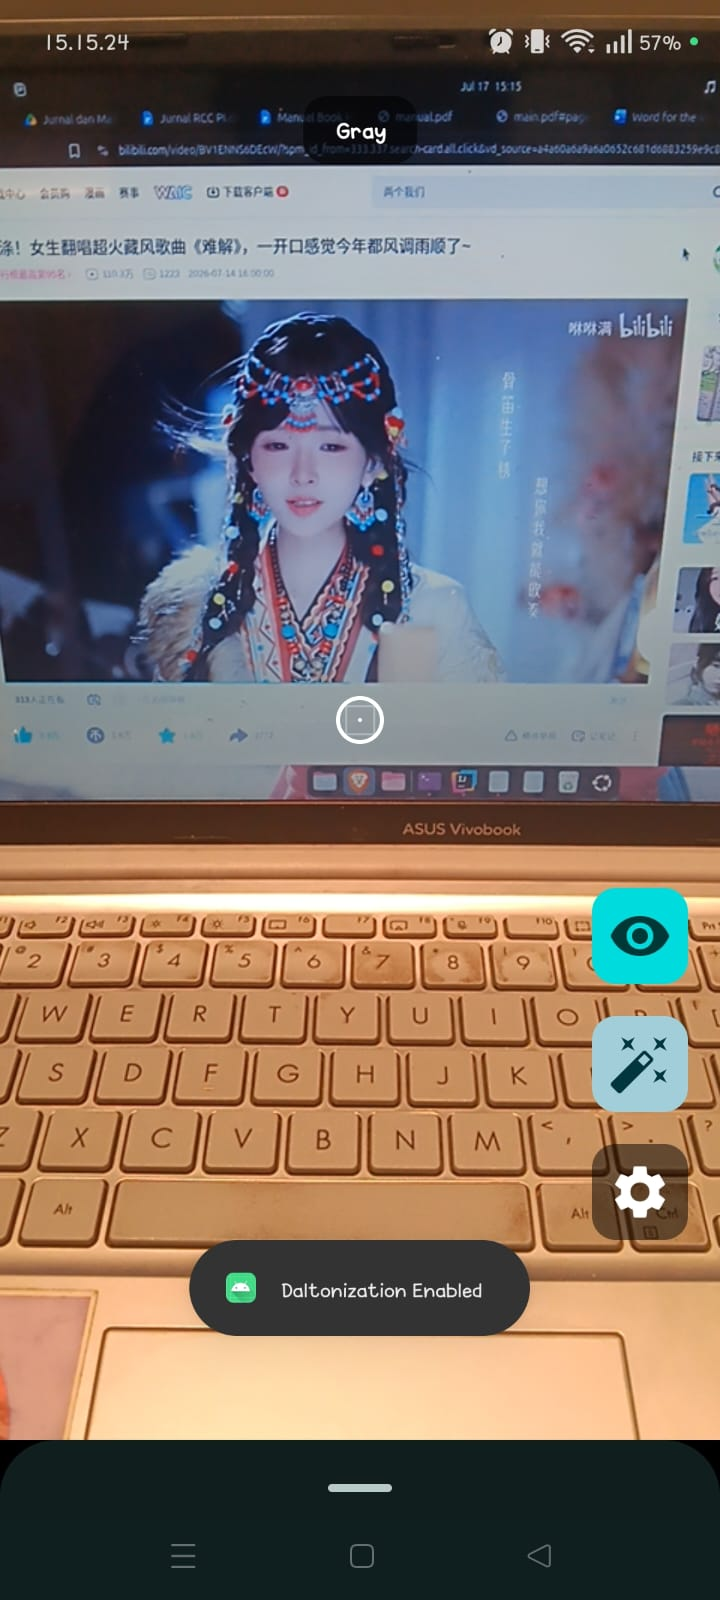
\includegraphics[width=\linewidth]{4}\\[0.2em]
  \textit{Notifikasi setelah filter diaktifkan}
\end{minipage}
\vspace{1em}

\item Mengaktifkan/Menonaktifkan Filter (ikon \textit{mata}): ikon mata
      pada sisi kanan layar berfungsi sebagai sakelar utama untuk
      mengaktifkan atau menonaktifkan seluruh filter. Saat dimatikan,
      tampilan kamera kembali normal tanpa efek apa pun, terlepas dari
      pengaturan Simulation Type atau Daltonisasi yang telah dipilih
      pada Filter Settings. Saat diaktifkan, kamera menampilkan efek
      sesuai pengaturan yang sedang dipilih.

\noindent
\begin{minipage}[t]{0.48\linewidth}
  \centering
  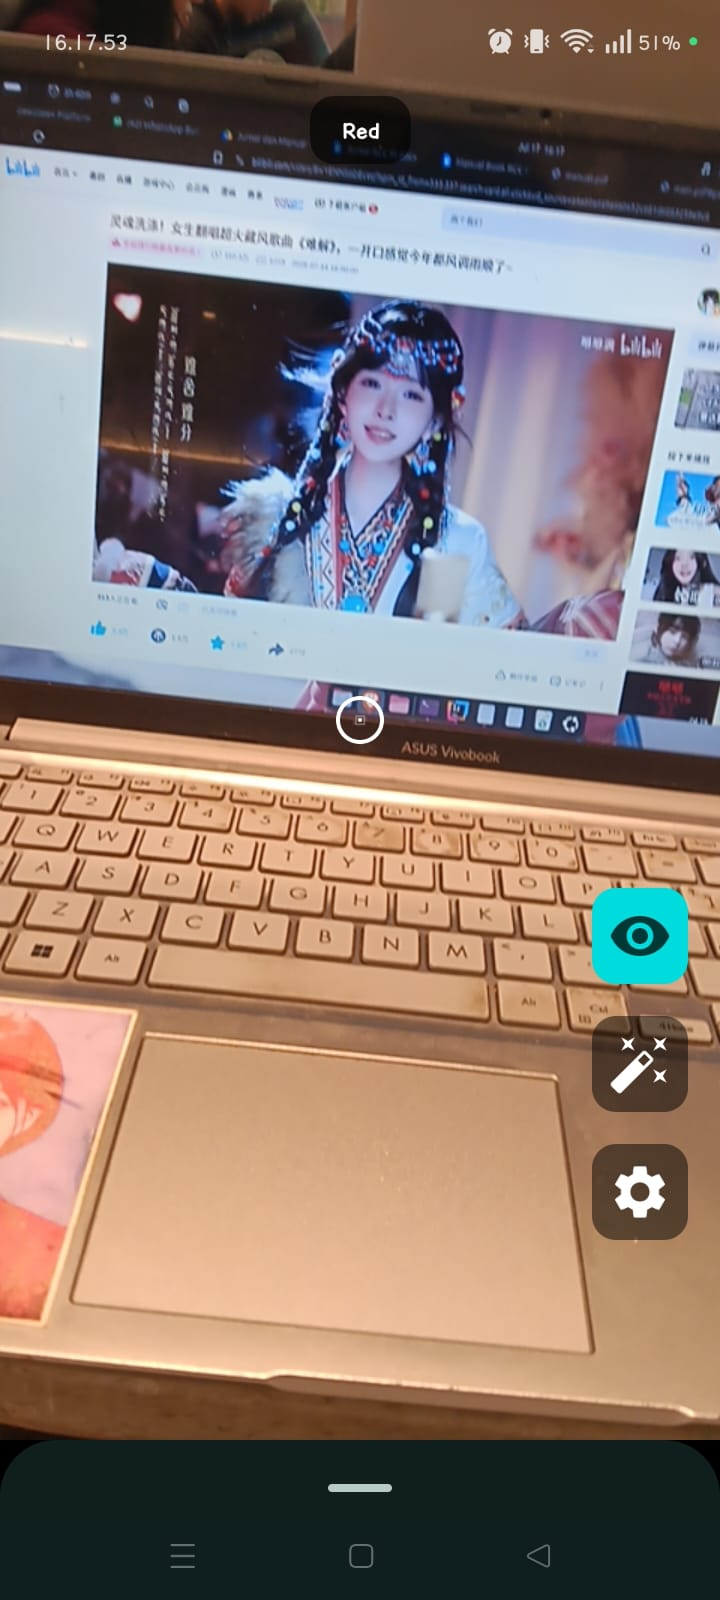
\includegraphics[width=\linewidth]{normal}\\[0.2em]
  \textit{Filter nonaktif (tampilan Normal)}
\end{minipage}
\hfill
\begin{minipage}[t]{0.48\linewidth}
  \centering
  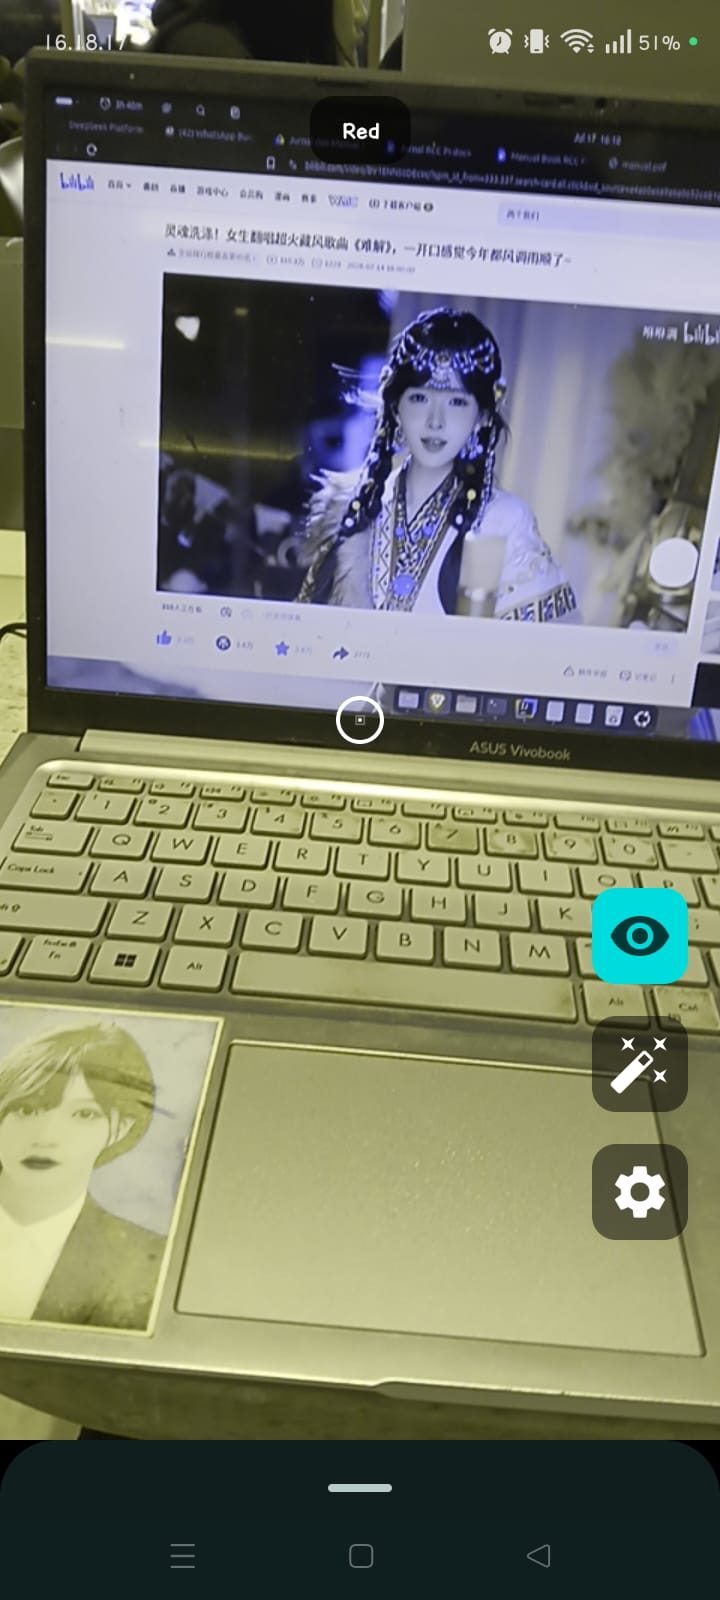
\includegraphics[width=\linewidth]{deut}\\[0.2em]
  \textit{Filter aktif (Simulation Type: Deuteranopia)}
\end{minipage}
\vspace{1em}

\item Mengatur Simulasi dan Daltonisasi (ikon \textit{tongkat sihir}):
      ketuk ikon tongkat sihir untuk membuka panel \textbf{Filter
      Settings}, tempat pengguna memilih \textbf{Simulation Type}
      (Normal, Protanopia, Deuteranopia, atau Tritanopia) yang
      memperlihatkan bagaimana sebuah objek terlihat bagi penderita
      dikromasi, sekaligus mengaktifkan \textbf{Enable Daltonization}
      untuk menerapkan koreksi warna di atas simulasi yang sedang
      dipilih. Fitur Daltonisasi menggeser informasi warna yang hilang
      akibat dikromasi ke spektrum warna lain yang lebih mudah
      dibedakan.

\noindent
\begin{minipage}[t]{0.48\linewidth}
  \centering
  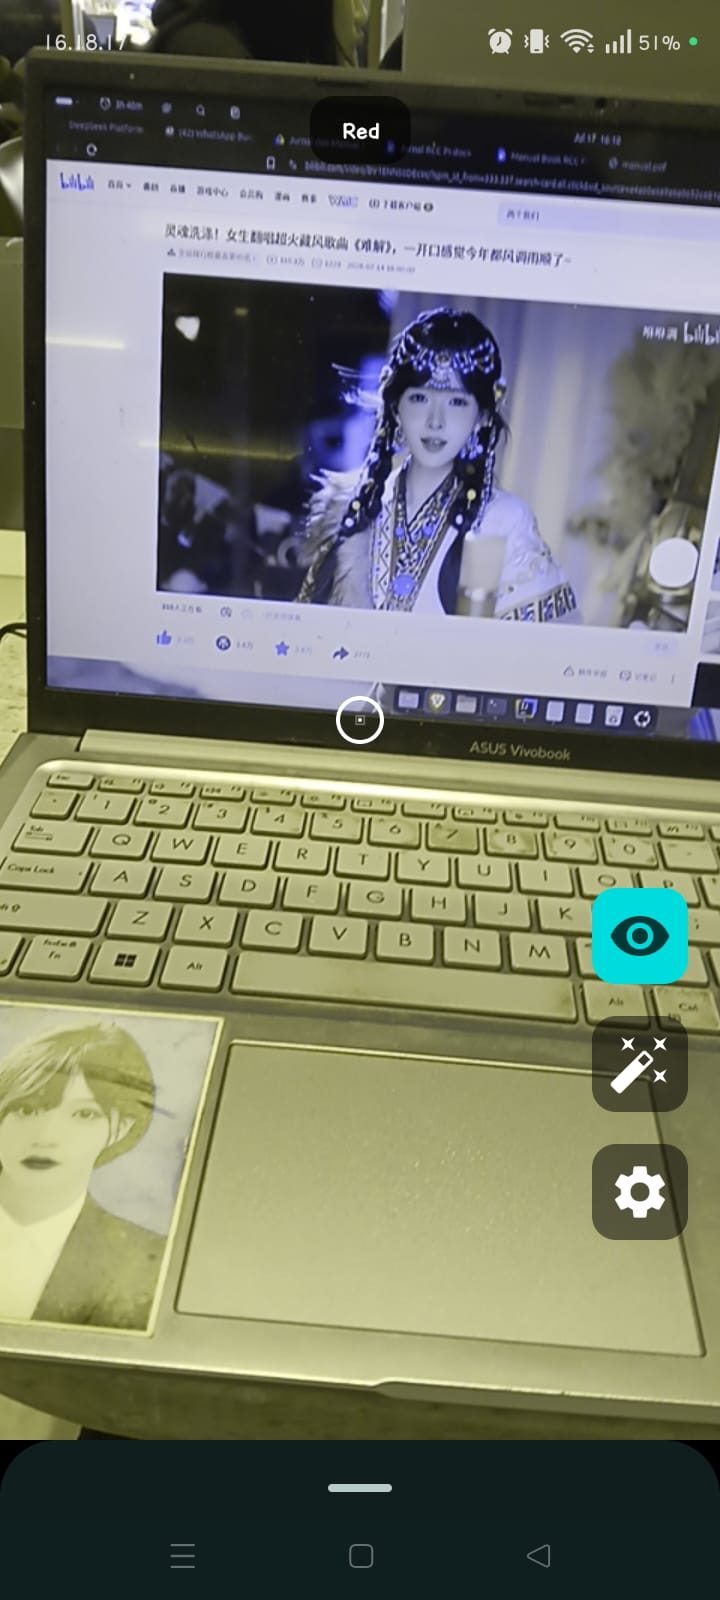
\includegraphics[width=\linewidth]{deut}\\[0.2em]
  \textit{Simulasi Deuteranopia (Daltonisasi nonaktif)}
\end{minipage}
\hfill
\begin{minipage}[t]{0.48\linewidth}
  \centering
  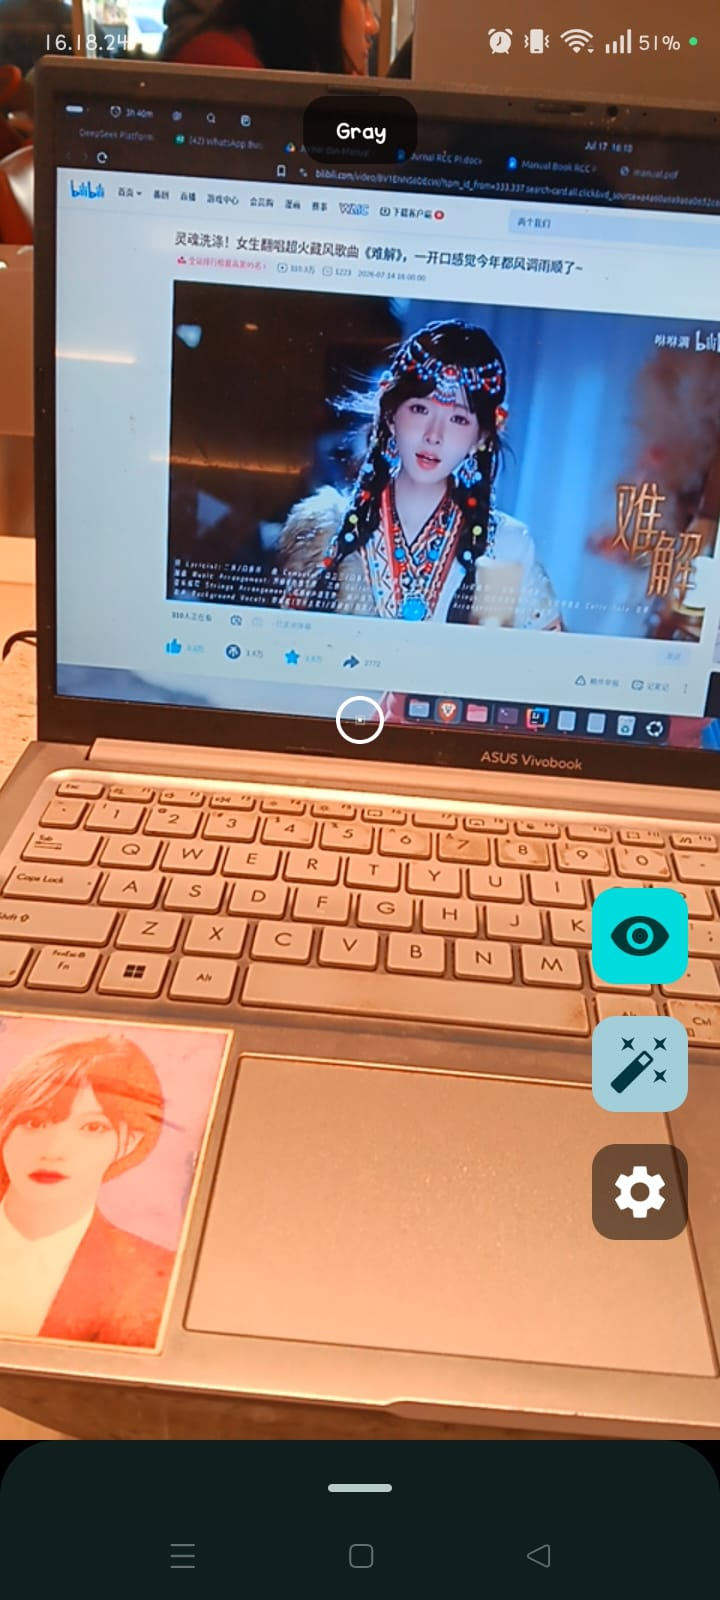
\includegraphics[width=\linewidth]{deut_dalt}\\[0.2em]
  \textit{Simulasi Deuteranopia + Daltonisasi aktif}
\end{minipage}
\vspace{1em}

Dengan Daltonisasi aktif, warna pada objek digeser ke rona biru dan
oranye yang lebih kontras dibandingkan tampilan Simulasi murni,
sehingga membantu penderita Deuteranopia membedakan objek yang tadinya
tampak serupa.

\item Alat Bantu Identifikasi Warna (\textit{Color Classification
      Test}): halaman ini merupakan alat bantu pengambilan sampel warna
      dari kamera, dapat diakses melalui menu \textit{Color
      Classification Test} pada halaman \textit{Dashboard}. Fitur yang
      tersedia antara lain:
\begin{itemize}
  \item Menampilkan nama warna (misalnya \textit{Red}, \textit{Green},
        \textit{Blue}, dan sebagainya) dari objek pada titik tengah
        layar secara \textit{real-time}.
  \item Menampilkan nilai warna hasil sampel dalam format RGB, HSV, dan
        HEX sekaligus.
  \item Mengubah (\textit{edit}) nilai RGB/HSV/HEX tersebut secara
        manual untuk melihat pratinjau warna yang dihasilkan.
  \item Membandingkan warna yang ditangkap kamera dengan warna lain
        pilihan pengguna.
  \item Memanipulasi nilai warna yang telah diambil sesuai kebutuhan
        pengujian.
\end{itemize}

\item Interpretasi Hasil: hasil deteksi warna, sampel RGB/HSV/HEX, dan
      filter daltonisasi bersifat sebagai alat bantu visual, bukan alat
      diagnosis medis. Pengguna yang mencurigai adanya gangguan
      penglihatan warna tetap disarankan untuk berkonsultasi dengan
      dokter mata atau tenaga medis profesional.

\end{enumerate}
\end{enumerate}

\end{document}
